\documentclass[english,10pt, compress]{beamer}
%\documentclass[english,10pt, compress, handout]{beamer}
\usepackage{mathptmx}
\usepackage[T1]{fontenc}
\usepackage[latin9]{inputenc}
\usepackage{color}
\usepackage{array}
\usepackage{multirow}
\usepackage{amsmath}
\usepackage{amssymb}
\usepackage{fancyvrb}
\usepackage{multicol}
\usepackage{rotating}
\makeatletter

%%%%%%%%%%%%%%%%%%%%%%%%%%%%%% LyX specific LaTeX commands.
\newcommand{\noun}[1]{\textsc{#1}}
%% Because html converters don't know tabularnewline
\providecommand{\tabularnewline}{\\}

%%%%%%%%%%%%%%%%%%%%%%%%%%%%%% Textclass specific LaTeX commands.
 % this default might be overridden by plain title style
 \newcommand\makebeamertitle{\frame{\maketitle}}%
 \AtBeginDocument{
   \let\origtableofcontents=\tableofcontents
   \def\tableofcontents{\@ifnextchar[{\origtableofcontents}{\gobbletableofcontents}}
   \def\gobbletableofcontents#1{\origtableofcontents}
 }
 \long\def\lyxframe#1{\@lyxframe#1\@lyxframestop}%
 \def\@lyxframe{\@ifnextchar<{\@@lyxframe}{\@@lyxframe<*>}}%
 \def\@@lyxframe<#1>{\@ifnextchar[{\@@@lyxframe<#1>}{\@@@lyxframe<#1>[]}}
 \def\@@@lyxframe<#1>[{\@ifnextchar<{\@@@@@lyxframe<#1>[}{\@@@@lyxframe<#1>[<*>][}}
 \def\@@@@@lyxframe<#1>[#2]{\@ifnextchar[{\@@@@lyxframe<#1>[#2]}{\@@@@lyxframe<#1>[#2][]}}
 \long\def\@@@@lyxframe<#1>[#2][#3]#4\@lyxframestop#5\lyxframeend{%
   \frame<#1>[#2][#3]{\frametitle{#4}#5}}
 \newenvironment{topcolumns}{\begin{columns}[t]}{\end{columns}}
 \def\lyxframeend{} % In case there is a superfluous frame end


%\setbeamersize{text margin left=.5cm, text margin right=.5cm, text}
% I personally don't think the navigation symbols add anything useful

\hypersetup{colorlinks, urlcolor=blue, linkcolor=magenta}

\usetheme{Warsaw}

\DeclareRobustCommand{\CC}{\hbox{C\hspace{-0.5ex}
                       \protect\raisebox{0.5ex}
                       {\protect\scalebox{0.67}{++}}}}


%\setbeamertemplate{headline}
%{%
%\begin{beamercolorbox}{section in head/foot}
%%\vskip2pt\insertnavigation{\paperwidth}\vskip2pt
%\end{beamercolorbox}%
%}

\newcommand{\Emph}[1]{\textcolor{magenta}{{#1}}}


\usefonttheme{serif}
%\usefonttheme{stillsanserifsmall}
\setbeamercovered{transparent}

\makeatother

\usepackage{babel}
\begin{document}


% Turn on pause for all items?
\beamerdefaultoverlayspecification{<+->}




\title[Move Semantics]{Move Semantics and RValue References}


\subtitle{Modern Software Engineering with \CC}


\author[SciTec]{Dave~Steffen}
\titlegraphic{
\includegraphics[scale=0.1]{SciTecLogo.jpeg}}

%\institute{}


%\date[]{}

\makebeamertitle






\AtBeginSubsection[]{

  \frame<beamer>{

    \frametitle{Outline}

    \tableofcontents[currentsection,currentsubsection]

  }

}



%\beamerdefaultoverlayspecification{<+->}


\lyxframeend{}\lyxframe{Outline}

\tableofcontents{}




\lyxframeend{}

%%%%%%%%%%%%%%%%%%%%%%%%%%%%%%%%%%%%%%%%%%%%%%%%%%%%%%%%%%%%%%%%%%%%%%
%%%%%%%%%%%%%%%%    SLIDES     %%%%%%%%%%%%%%%%%%%%%%%%%%%%%%%%%%%%%%%
%%%%%%%%%%%%%%%%%%%%%%%%%%%%%%%%%%%%%%%%%%%%%%%%%%%%%%%%%%%%%%%%%%%%%%



\begin{frame}[fragile,t]
\frametitle{Dynamic Memory Is Hard}
\framesubtitle{``If you write C-style code, you expect to have C-style problems'' -- Stroustrup}

{\scriptsize \begin{verbatim}
void foo() {
  double* d = new double[70];
  ...
  if (condition1)
    return;       // Leak!
  ...
  if (error)
    throw ex;     // Leak!

  foo()           // if an exception happens
                  // in here -- Leak!

  delete d;      // cleanup (?)
}
\end{verbatim}}
\end{frame}




%%%%%%%%%%%%%%%%%%%%%%%%%%%%%%%%%%%%%%%%%%%%%%%%%%%%%%%%%%%%%%%%%%%%%%
\begin{frame}[fragile,t]
\frametitle{SESE}

Single-Entry-Single-Exit is an attempt to mitigate this problem:

\begin{columns}[t]
\column{.5\textwidth}
Heavily nested if-blocks:
{\scriptsize\begin{verbatim}
void foo() {
  if (precondition1) {
    double* d = new double[70];
    if (d) {
      ...
      if (precondition2) {
        Widget* w = new Widget;
        if (w) {
           // finally do some work
           FiddleWidget(w);
           ...
           }
        delete w;
        }
     }
   delete d[];
   }
  return;
}
\end{verbatim}}
\pause{}
\column{.5\textwidth}
And doesn't help anyway
{\scriptsize\begin{verbatim}


// Can throw in C++11



// ... might throw



// might throw






\end{verbatim}}
\end{columns}
\pause{}
In the presence of exceptions, \Emph{every function call} can exit the function
\end{frame}


%%%%%%%%%%%%%%%%%%%%%%%%%%%%%%%%%%%%%%%%%%%%%%%%%%%%%%%%%%%%%%%%%%%%%%

\begin{frame}[fragile,t]
\frametitle{Exceptions Break Things}
\framesubtitle{If you don't know what you're doing}
In the presence of exceptions, writing code the old way is nearly impossible:
{\scriptsize\
\begin{verbatim}
void foo() {
  try {  double* d = new double[70]; }
  catch (...) {...}
  ...
  try { foo(); }
  catch (...) { delete d; ...}

  try { bar(); } 
  catch (...) { delete d; ...}

  delete d;      // cleanup
}
\end{verbatim}
}
Every statement must be wrapped in a try/catch block... this is part of the reason exceptions have a bad rap in C++.
\end{frame}

%%%%%%%%%%%%%%%%%%%%%%%%%%%%%%%%%%%%%%%%%%%%%%%%%%%%%%%%%%%%%%%%%%%%%%

\begin{frame}[fragile,t]
\frametitle{}
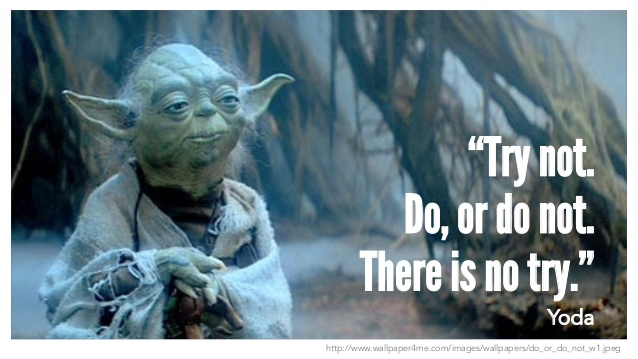
\includegraphics[scale=0.5]{yoda.jpg}

Many (most?) C++ code bases \emph{do not use exceptions}, including
Google's, and including ours.

Writing code \emph{as if} in the presence of exceptions makes code better.

\end{frame}

\begin{frame}[fragile,t]
\frametitle{A Rant}
\framesubtitle{Before we go on...}
There is something very wrong here:
\pause{}
{\scriptsize \begin{verbatim}
void foo() {

  Widget* w = new Widget;
  ...
  if (condition1)
    return;       // Leak!
  ...
  if (error)
    throw ex;     // Leak!

  foo()           // an exception happens
                  // in here -- Leak!

  delete w;      // cleanup 
}
\end{verbatim}}
\pause
\Emph{This isn't Java, so stop it.}

\end{frame}

\begin{frame}[fragile,t]
\frametitle{A Rant}
\framesubtitle{Before we go on...}
Don't hit the heap if you don't have to!

{\scriptsize \begin{verbatim}
void foo() {

  Widget w;      // On the stack!
  ...
  if (condition1)
    return;       // nothing to leak
  ...
  if (error)
    throw ex;     // no problems

  foo()           // an exception happens in here... ok
}
\end{verbatim}}
\pause{}
\begin{itemize}
\item Save runtime
\item Reduce pressure on the heap
\item Reduce memory fragmentation
\pause{}
\item \Emph{Repent, ye Java programmers}
\end{itemize}

\end{frame}

%%%%%%%%%%%%%%%%%%%%%%%%%%%%%%%%%%%%%%%%%%%%%%%%%%%%%%%%%%%%%%%%%%%%%%%%%%%%%%%%

\begin{frame}[fragile,t]
\frametitle{Why dynamic memory at all?}
\center{When must we hit the heap?}
\vskip 6pt
\pause{}

\begin{enumerate}
\item We don't know how many we need until runtime
{\scriptsize \begin{verbatim}
int n;
cin >> n;
Widget* widgets = new Widget[n];
\end{verbatim}
}
\pause{}
\item We don't know what type we need until runtime (polymorphism)
{\scriptsize \begin{verbatim}
class DooDad : public Widget {};
class DooHickey : public DooDad {};
class Gadget : public Widget{}
class Thingy : public Gadget{};

Widget* widget = WidgetFactory(...);
\end{verbatim}
}
\pause{}
\item We don't know how long it's going to live (special case of \#1)
\end{enumerate}

\vskip 12pt
\pause{}

\center{ \Emph{Dynamically allocate only when absolutely necessary} }
\end{frame}



\subsection{\&\& / Move}\lyxframeend{}

%%%%%%%%%%%%%%%%%%%%%%%%%%%%%%%%%%%%%%%%%%%%%%%%%%%%%%%%%%%%%%%%%%%%%%
%%%%%%%%%%%%%% auto 1

\begin{frame}[fragile,t]
\frametitle{Copies Are The Problem}

\begin{itemize}

\item{\scriptsize
\begin{verbatim}
vector<string> get_names() {... return m_names;} // #1
vector<string> names = get_names(); // #2
\end{verbatim}
}

\item In principle, two copies of the vector, and a default constructor.

\item If there are N strings in the vector, each copy could require as many
as N+1 memory allocations and a whole slew of cache-unfriendly data
accesses as the string contents are copied.


\vskip 12pt
\item Option 1: don't ever change the result
{\scriptsize
\begin{verbatim}
vector<string> const& names = get_names();
\end{verbatim}
}

\vskip 12pt

\item Option 2: commit to smart pointers
{\scriptsize
\begin{verbatim}
shared_ptr<vector<string>> get_names();
\end{verbatim}
}
\vskip 12pt

\item Option 3: FORTRAN-style ``out parameters''
{\scriptsize
\begin{verbatim}
void get_names( vector<string>& m_names);
\end{verbatim}
}


\end{itemize}

\end{frame}

%%%%%%%%%%%%%%%%%%%%%%%%%%%%%%%%%%%%%%%%%%%%%%%%%%%%%%%%%%%%%%%%%%%%%%

\begin{frame}[fragile,t]
\frametitle{Copies Are Inevitable}
{\scriptsize
\begin{verbatim}
class Vector {...};

Vector operator+ (Vector const& A, Vector const& B) {
  Vector result(A);
  return result += B;
}
...
Vector C =    A + B  + D  + Foo(E+F);
   --->  = (((A + B) + D) + Foo(E+F));
\end{verbatim}
}

\begin{itemize}
\item Five subexpressions means five unnamed temporaries, means five
  copies, and then the assignment.
\item Options 2 and 3 are not an option unless we give up the syntax.
\item Option 1 doesn't help and may not be a viable option anyway.
\end{itemize}

\uncover<2>{ \hfill \textcolor{purple} {Copies are the bane of
    high-performance computing in \CC.} \hfill}


\end{frame}

%%%%%%%%%%%%%%%%%%%%%%%%%%%%%%%%%%%%%%%%%%%%%%%%%%%%%%%%%%%%%%%%%%%%%%

\begin{frame}[fragile,t]
\frametitle{Compilers aren't that stupid}

\textcolor{red}{Copy Elision to the rescue!}

\begin{itemize}
\item<1-> All modern compilers make these the same:
{\scriptsize
\begin{verbatim}
vector<string> names = get_names();
vector<string> names(get_names);
\end{verbatim}}

\item<1->Return Value Optimization (RVO):{\scriptsize
\begin{verbatim}
vector<string> get_names() {
  vector<string> result;
  ...
  return result; } 

  vector<string> names = get_names();
\end{verbatim}}

\item<1->''Unnamed RVO'':{\scriptsize
\begin{verbatim}
vector<string> get_names() {
  string twoB, not2B;
  ...
  return twoB + " or " + not2B; } 

  vector<string> names = get_names();
\end{verbatim}}

\textcolor{red}{Compilers can skip copy operations \emph{if doing so
    has no observable effects}.}
\end{itemize}
\end{frame}

\begin{frame}[fragile,t]
\frametitle{... but compilers are limited}

\textcolor{red}{Copy elision is fragile}


\begin{itemize}
\item<1-> Copy elision not allowed if these have side effects:
{\scriptsize
\begin{verbatim}
vector<string> names = get_names();
vector<string> names(get_names);
\end{verbatim}
}

\item<1-> NRVO / URVO happens, on a compiler-by-compiler basis.
\item<1-> RVO is easily disabled in compiler specific ways:
{\scriptsize
\begin{verbatim}
Foo makefoo() {
  Foo a;
  ...
  if (expr) return a;
  ...
  return b;
}
\end{verbatim}
}
\end{itemize}

\textcolor{red}{Copy elision happens at the whim of the compiler, and
  there's not much you can do to help.}
\end{frame}



\begin{frame}[fragile]
\frametitle{Enter Move Semantics}

In all these cases we don't want a copy: \emph{we're never going to
  use the original again!}

\begin{verbatim}
Vector C =    A + B  + D  + Foo(E+F);
\end{verbatim}


``We aren't going to use this object again'' has a name:

\uncover<2->{ \hfill \textcolor{purple} {rvalue reference, spelled \&\&} \hfill}
\uncover<3>{

\begin{itemize}
\item {\bf lvalue}: can appear on the left side of an assignment
\item[] EG: variables \note{const objects are lvalues!}
\item {\bf rvalues} : can \emph{only} appear on the right side of an assignment
\item[] EG: literals, unnamed temporaries
\end{itemize}
}

\end{frame}
%%%%%%%%%%%%%%%%%%%%%%%%%%%%%%%%%%%%%%%%%%%%%%%%%%%%%%%%%%%%%%%%%%%%%%
\begin{frame}[fragile]
\frametitle{rvalues}

Unnamed temporaries can only be referenced (viewed) once.  Therefore,
they can be organ donors.

{\scriptsize
\begin{verbatim}
class A {
  A( const A& lvalue };          // copy ctor
  A& operator=(const A& lvalue)  // copy assignment
  A( A&& rvalue );               // move ctor
  A& operator=(A&& rvalue);      // move assignment

  shared_ptr<Foo> r;
}
\end{verbatim}
}

Move: steal the guts from the organ donor.

{\scriptsize
\begin{verbatim}
A::A( A&& rvalue ) : r(rvalue.r) {}
\end{verbatim}
}
Usage:
{\scriptsize
\begin{verbatim}
A make_an_A();
...A a;
...
a = make_an_A();
\end{verbatim}
}
No Copies!
\end{frame}

%%%%%%%%%%%%%%%%%%%%%%%%%%%%%%%%%%%%%%%%%%%%%%%%%%%%%%%%%%%%%%%%%%%%%%

\begin{frame}[fragile]
\frametitle{Moving Vectors}
{\scriptsize
\begin{verbatim}
class Vector {
  double* data;   int len;

  Vector(Vector&& rref) : data(rref.data), len(rref.data)  {
    rref.m_data = nullptr;
  }

  Vector& operator=(Vector&& rref) {
    swap(data, rref.data)
    len  = rref.len;
  }

  ~Vector() { delete[] m_data; }

};


Vector C =    A + B  + D  + Foo(E+F);

\end{verbatim}
}

Moved-from objects are in an \emph{inconsistent} but
\emph{destructable} state.

\end{frame}

%%%%%%%%%%%%%%%%%%%%%%%%%%%%%%%%%%%%%%%%%%%%%%%%%%%%%%%%%%%%%%%%%%%%%%

\begin{frame}[fragile]
\frametitle{std::move}
Force a move from something that isn't an rvalue already:
{\scriptsize
\begin{verbatim}

Vector V;

...

Vector Q = std::move(V);

// don't use V again!

cout << V.len;  // undefined behavior!

\end{verbatim}
}

\end{frame}

%%%%%%%%%%%%%%%%%%%%%%%%%%%%%%%%%%%%%%%%%%%%%%%%%%%%%%%%%%%%%%%%%%%%%%

\begin{frame}[fragile]
\frametitle{Coding move assignments}
\begin{enumerate}
\item Swap resources. Cleaner, faster?
{\scriptsize
\begin{verbatim}
class Vector {
  double* data;

  Vector& operator=(Vector&& rref) {
    swap(data, rref.data)
  }

  ~Vector() { delete[] m_data; }
};
\end{verbatim}
}
\item Delete the unneeded resources directly; deterministic, necessary?
{\scriptsize
\begin{verbatim}
class Vector {
  ...

  Vector& operator=(Vector&& rref) {
    delete[] data;
    data = rref.data;
    rref.data = nullptr;
  }
};
\end{verbatim}
}
\end{enumerate}

The debate continues.
\end{frame}

%%%%%%%%%%%%%%%%%%%%%%%%%%%%%%%%%%%%%%%%%%%%%%%%%%%%%%%%%%%%%%%%%%%%%%

\begin{frame}[fragile]
\frametitle{Writing Functions}
\begin{itemize}
\item Return values?  As usual.
{\scriptsize
\begin{verbatim}
// Do this:               Not this!

Foo bar() {             Foo&& bar() {
  Foo f;                  Foo f;
  ...                     ...
  return f;               return f;
}                       }

\end{verbatim}
}
\item Pass by value when you want a copy.
{\scriptsize
\begin{verbatim}
void foo ( const bar& b) {  // not this
  bar local = b;
  // ... modify local
}

void foo ( bar b ) {        // but this
 // ... modify local b
\end{verbatim}
}
\end{itemize}

\end{frame}


%%%%%%%%%%%%%%%%%%%%%%%%%%%%%%%%%%%%%%%%%%%%%%%%%%%%%%%%%%%%%%%%%%%%%%

\begin{frame}[fragile]
\frametitle{Writing Functions II: Binding}
{\scriptsize
\begin{verbatim}
void Foo (const A& a, A& b, A c, A&& d)
{
  // a: lvalue,    const-ref to external l-or-rvalue
  // b: lvalue,    ref to external l-or-rvalue
  // c: lvalue,    local copy
  // d: lvalue(!), ref to external rvalue

  A e // lvalue, local variable

  A&& r = bar(a,b); // lvalue(!) - rref to local rvalue
                    // semantically an lvalue
                    // but it's an organ donor

  // Return value options: choose one:

  return e;  // e is local, move enabled

  return r;  // same
  
  return d;            // d not local -- copy!
  return std::move(d); // move enabled

  return a;            // copy
  return std::move(a); // BOOM!
}
\end{verbatim}
}

\end{frame}



%%%%%%%%%%%%%%%%%%%%%%%%%%%%%%%%%%%%%%%%%%%%%%%%%%%%%%%%%%%%%%%%%%%%%%

\begin{frame}[fragile]
\frametitle{Writing Functions III}
{\scriptsize
\begin{verbatim}
Matrix operator+(Matrix const& x, Matrix const& y) // #1
{ Matrix temp = x; temp += y; return temp; }
 
Matrix operator+(Matrix&& temp, const Matrix& y)   // #2
{ temp += y; return std::move(temp); }
 
Matrix operator+(const Matrix& x, Matrix&& temp)   // #3
{ temp += x; return std::move(temp); }
 
Matrix operator+(Matrix&& temp, Matrix&& y)        // #4
{ temp += y; return std::move(temp); }
\end{verbatim}
}

\begin{itemize}
\item \#1 : Move enabled, because \texttt{temp} is an automatic
  variable: provably never used again!
\item \#2 -- \#4: Use \texttt{std::move} because \texttt{temp} is \emph{not}
  an automatic variable

\item A named rvalue reference is an lvalue! (It's not unnamed any
  more!) Inside \#2, \texttt{temp} is an lvalue reference.
\end{itemize}


\end{frame}


%%%%%%%%%%%%%%%%%%%%%%%%%%%%%%%%%%%%%%%%%%%%%%%%%%%%%%%%%%%%%%%%%%%%%%

\begin{frame}[fragile]
\frametitle{Coding move-enabled classes}
{\scriptsize
\begin{verbatim}
struct Widget {  

 std::string s;

  Widget(Widget&& rhs)
    : s(rhs.s)             // Incorrect!
   {...}

  Widget(Widget&& rhs)
    : s(std::move(rhs.s))  // Correct!
   {...}
\end{verbatim}
}
\begin{itemize}
\item Remember, binding an rvalue to something produces an lvalue (it
  has a name!); it's just an lvalue that you can cannibalize.
\end{itemize}

\end{frame}


%%%%%%%%%%%%%%%%%%%%%%%%%%%%%%%%%%%%%%%%%%%%%%%%%%%%%%%%%%%%%%%%%%%%%%

\begin{frame}[fragile]
\frametitle{Move rules of thumb}
\begin{itemize}
\item Leave moved-from objects in a destructable and assignable state.
\item Move operations preserve user-visible side effects on the LHS.
  (E.G., LHS's resources get released immediately.  General
  consensus?)
\item Return values from functions as values, not \&\& or any other
  wierd thing
\item Pass by value if you want a copy ('cause you might get a move!)
\item Tell the compiler you're done with an object with std::move()
\item These rules of thumb haven't quite been worked out -- see our
  coding standards for some other issues.
\item Remember: move is an optimization of copy, so all of the above
  can be ignored without any consequence worse than missed
  optimization opportunities.
\end{itemize}

\end{frame}


%%%%%%%%%%%%%%%%%%%%%%%%%%%%%%%%%%%%%%%%%%%%%%%%%%%%%%%%%%%%%%%%%%%%%%
\begin{frame}[fragile,t]
\frametitle{Summary}
\begin{itemize}[<+->]
\item \texttt{type\_traits.h} defines more type traits than would be
  wise to shake a stick at
\begin{itemize}
  \item Pay particular attention to \texttt{enable\_if}.
\end{itemize}
\item \cexpr is \emph{the} way to do compile-time value computations.
\begin{itemize}
  \item Prefer over recursive templates in all cases.
\end{itemize}
\item Variadic templates
\begin{itemize}
  \item \Emph{Wow}.  Or \Emph{Ouch}.  Or both.
\end{itemize}
\item Universal References and Perfect Forwarding.
\begin{itemize}
  \item Solutions to problems you didn't know you had (but you'd find
    out the hard way).
\end{itemize}
\end{itemize}
\end{frame}

%%%%%%%%%%%%%%%%%%%%%%%%%%%%%%%%%%%%%%%%%%%%%%%%%%%%%%%%%%%%%%%%%%%%%%
\begin{frame}[fragile,t]
\frametitle{Encouragement}
\begin{itemize}[<+->]
\item \Emph{This stuff is not academic}
\item Fundamental power-tools for library writers.
\item Fundamental power-tools for non-library writers.
\item Jason Turner: \CC17 game code for Commodore
  64. \url{https://www.youtube.com/watch?v=zBkNBP00wJE&t=1488s}
\vskip 6pt
\item A concern shared amongst many people in the Standards Committee:
\begin{itemize}
  \item People aren't thinking compile-time enough.
  \item Compile-time stuff is \emph{everywhere}
  \item Embedded work is \Emph{particularly} receptive / amenable /
    desperate for these techniques.
\end{itemize}
\end{itemize}
\pause
\vskip 24pt
\begin{center}
\Emph {Go Forth And Compile-Time Program!!!}
\end{center}
\end{frame}

%%%%%%%%%%%%%%%%%%%%%%%%%%%%%%%%%%%%%%%%%%%%%%%%%%%%%%%%%%%%%%%%%%%%%%
%% \begin{frame}[fragile,t]
%% \frametitle{}
%% \end{frame}







\end{document}
